\newpage
\section{Conclusion}
\label{sec:conclusion}

We can finally compare side by side the plots for the output voltages for the Envelope Detector and the Voltage Regulator, as well as the output AC component + DC deviation. 

Below we can see that the plots obtained are similar and any differences are within the expected discrepancy. Those can be due to the complexity and non-linearity of the used model, both theoretically and in the simulation. For the simulation deviation we obtained a value of 7.809000e-02 and as for theoretically we obtained a value of 1.5813e-01. These are also similar, making this laboratory considerably sucessful. Another reason for this can be the fact that we used the same values for $V_{on}, Is, \eta, V_{T}$ as Ngspice uses for the circuit model.

Finally, we can say we obtained a price of 72.15 and a merit of 1.774688e-01, values that were obtained through the already mentioned  optimization program that can be found in folder $mat$, which created a new Ngspice in each cycle, making sure that the value $n$ used for the transformer was well achieved throughout the required calculations and not a random number(since such assumption would drastically and wrongly improve the merit values).

\newpage
\begin{figure}[!ht] \centering
\caption{Simulation envelope detector voltage}
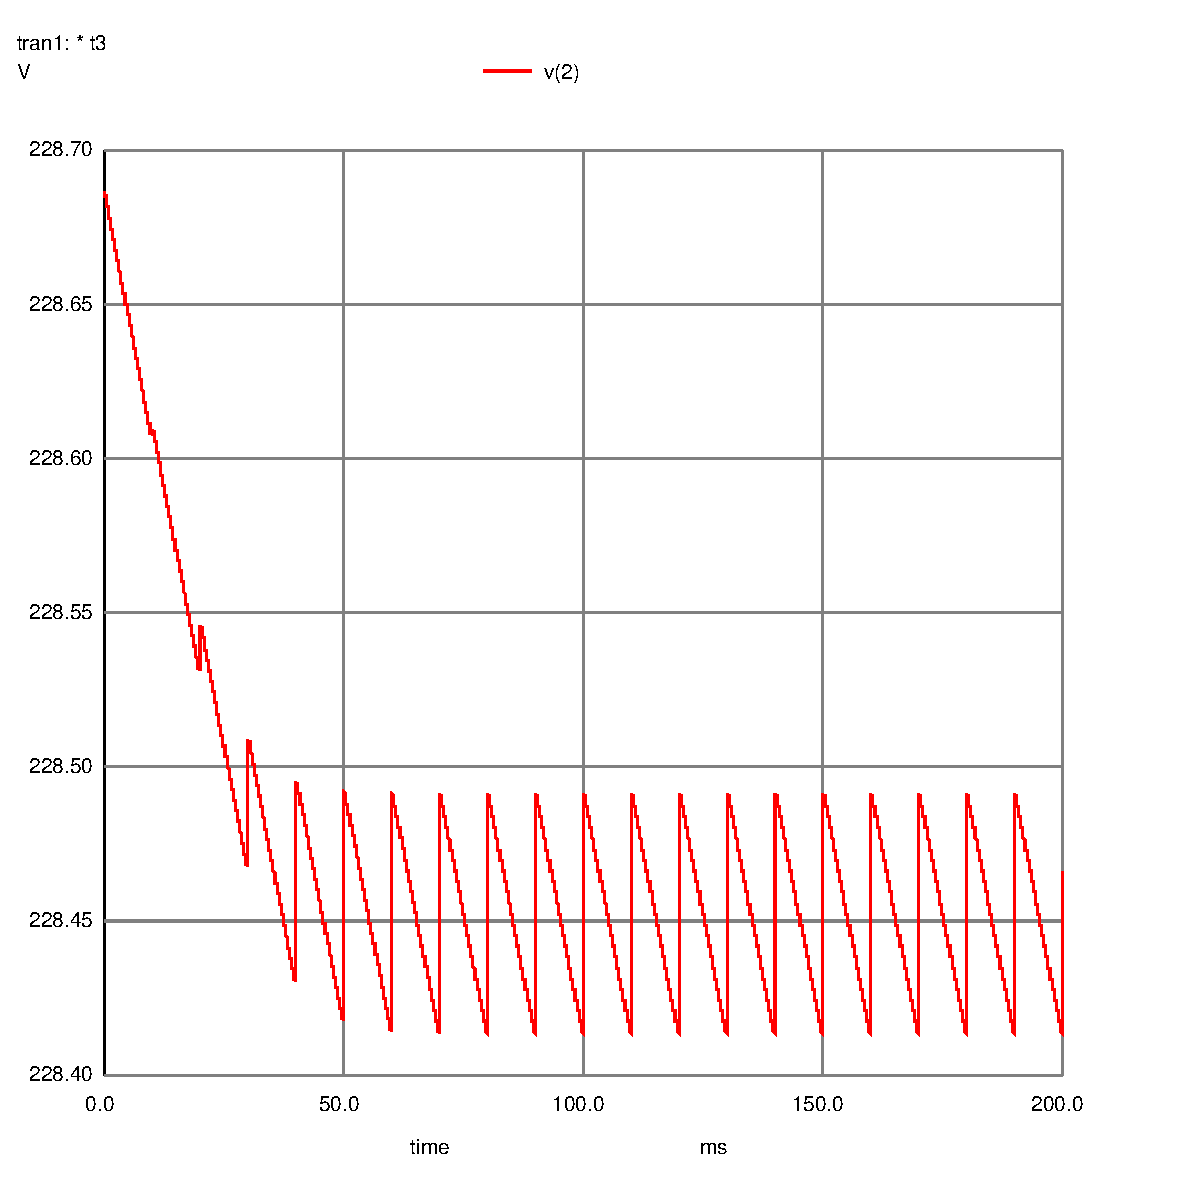
\includegraphics[width=0.6\linewidth]{venv.eps}
\label{fig:sim1}
\end{figure}

\begin{figure}[!ht] \centering
\caption{Theoretical envelope detector voltage}
\squeezeup 
\squeezeup 
\squeezeup 
\squeezeup 
\squeezeup 
\squeezeup 
\squeezeup 
\squeezeup 
\includegraphics[width=0.8\linewidth]{env_vout.pdf}
\label{fig:theo1}
\end{figure}

\begin{figure}[!ht] \centering
\caption{Simulation voltage regulator voltage}
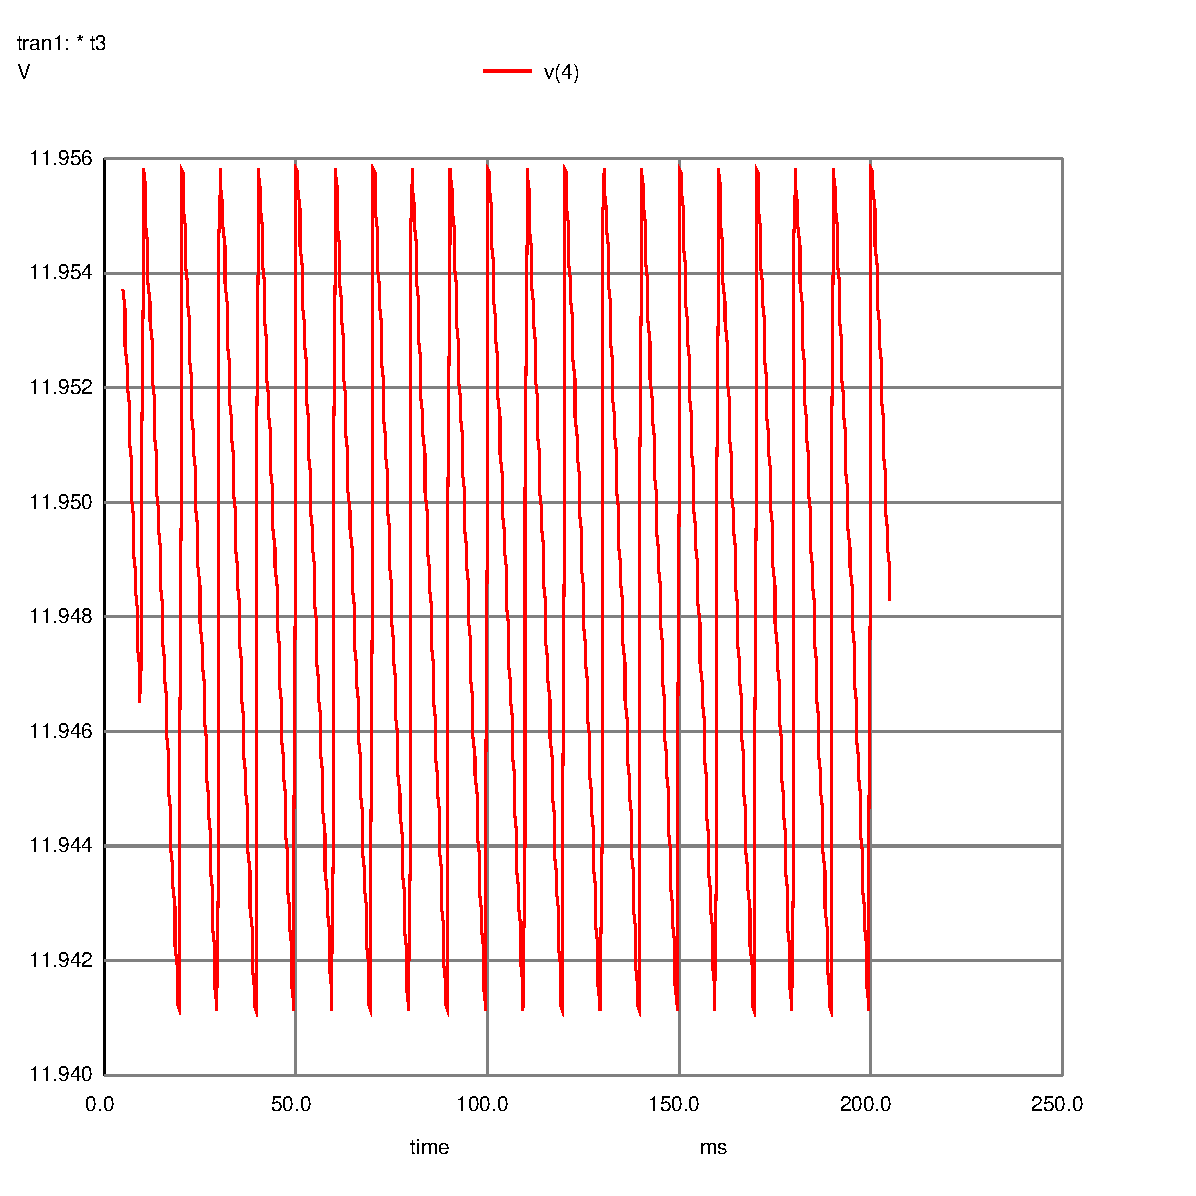
\includegraphics[width=0.6\linewidth]{vout.eps}
\label{fig:sim2}
\end{figure}


\begin{figure}[!ht] \centering
\caption{Theoretical voltage regulator voltage}
\squeezeup 
\squeezeup 
\squeezeup 
\squeezeup 
\squeezeup 
\squeezeup 
\squeezeup 
\squeezeup 
\includegraphics[width=0.8\linewidth]{t_vout.pdf}
\label{fig:theo2}
\end{figure}

\begin{figure}[!ht] \centering
\caption{Simulation output AC component + DC deviation}
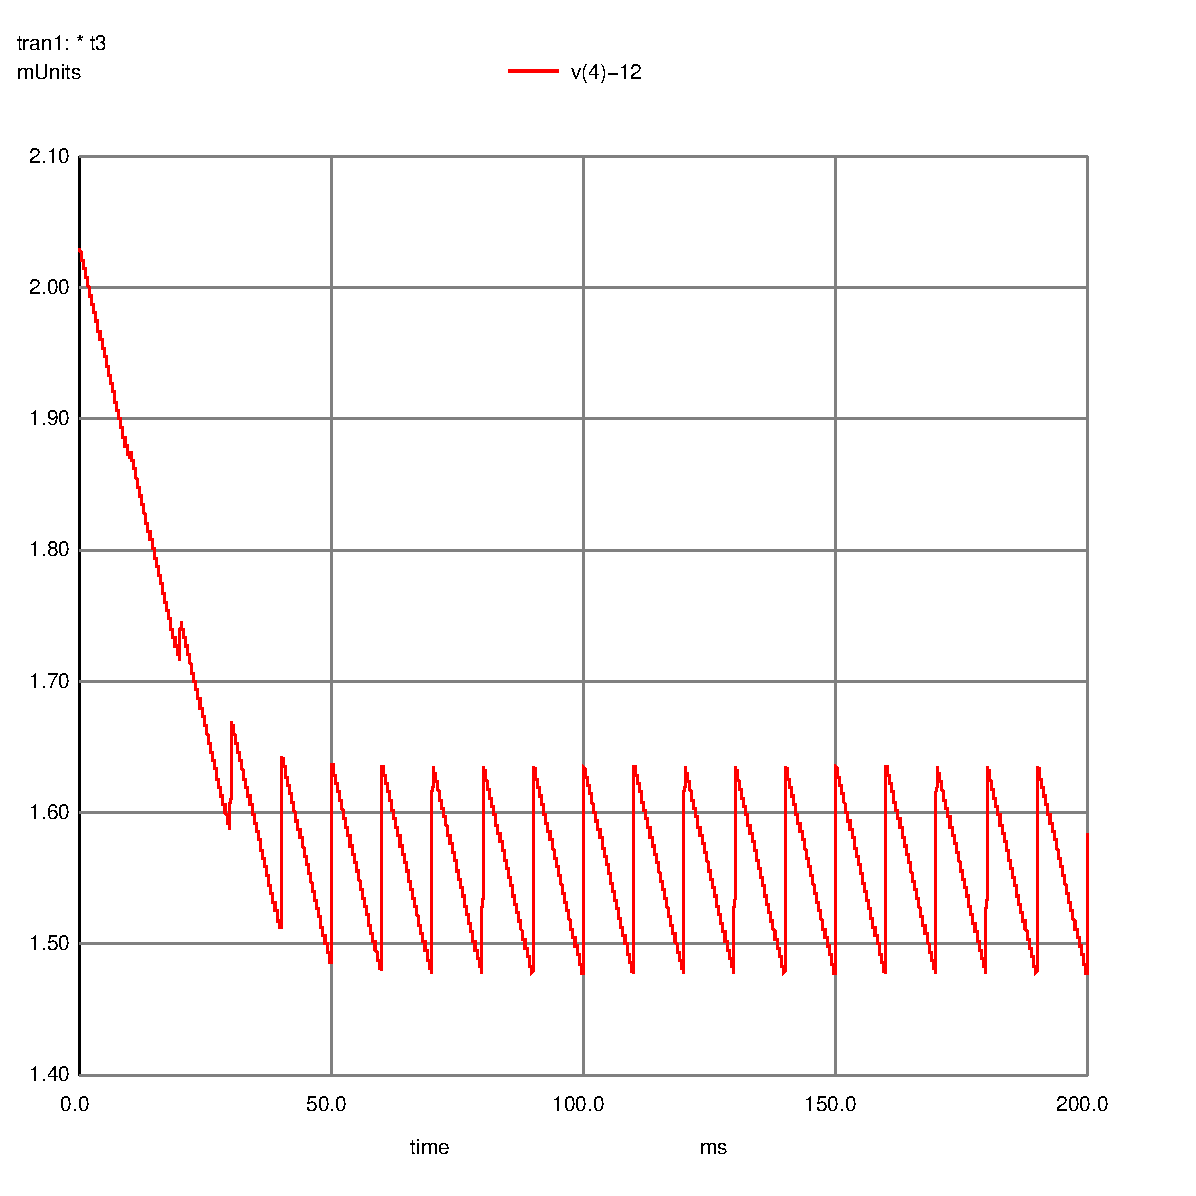
\includegraphics[width=0.6\linewidth]{vout(ac+dc).eps}
\label{fig:sim3}
\end{figure}

\begin{figure}[!ht] \centering
\caption{Theoretical output AC component + DC deviation}
\squeezeup 
\squeezeup 
\squeezeup 
\squeezeup 
\squeezeup 
\squeezeup 
\squeezeup 
\squeezeup 
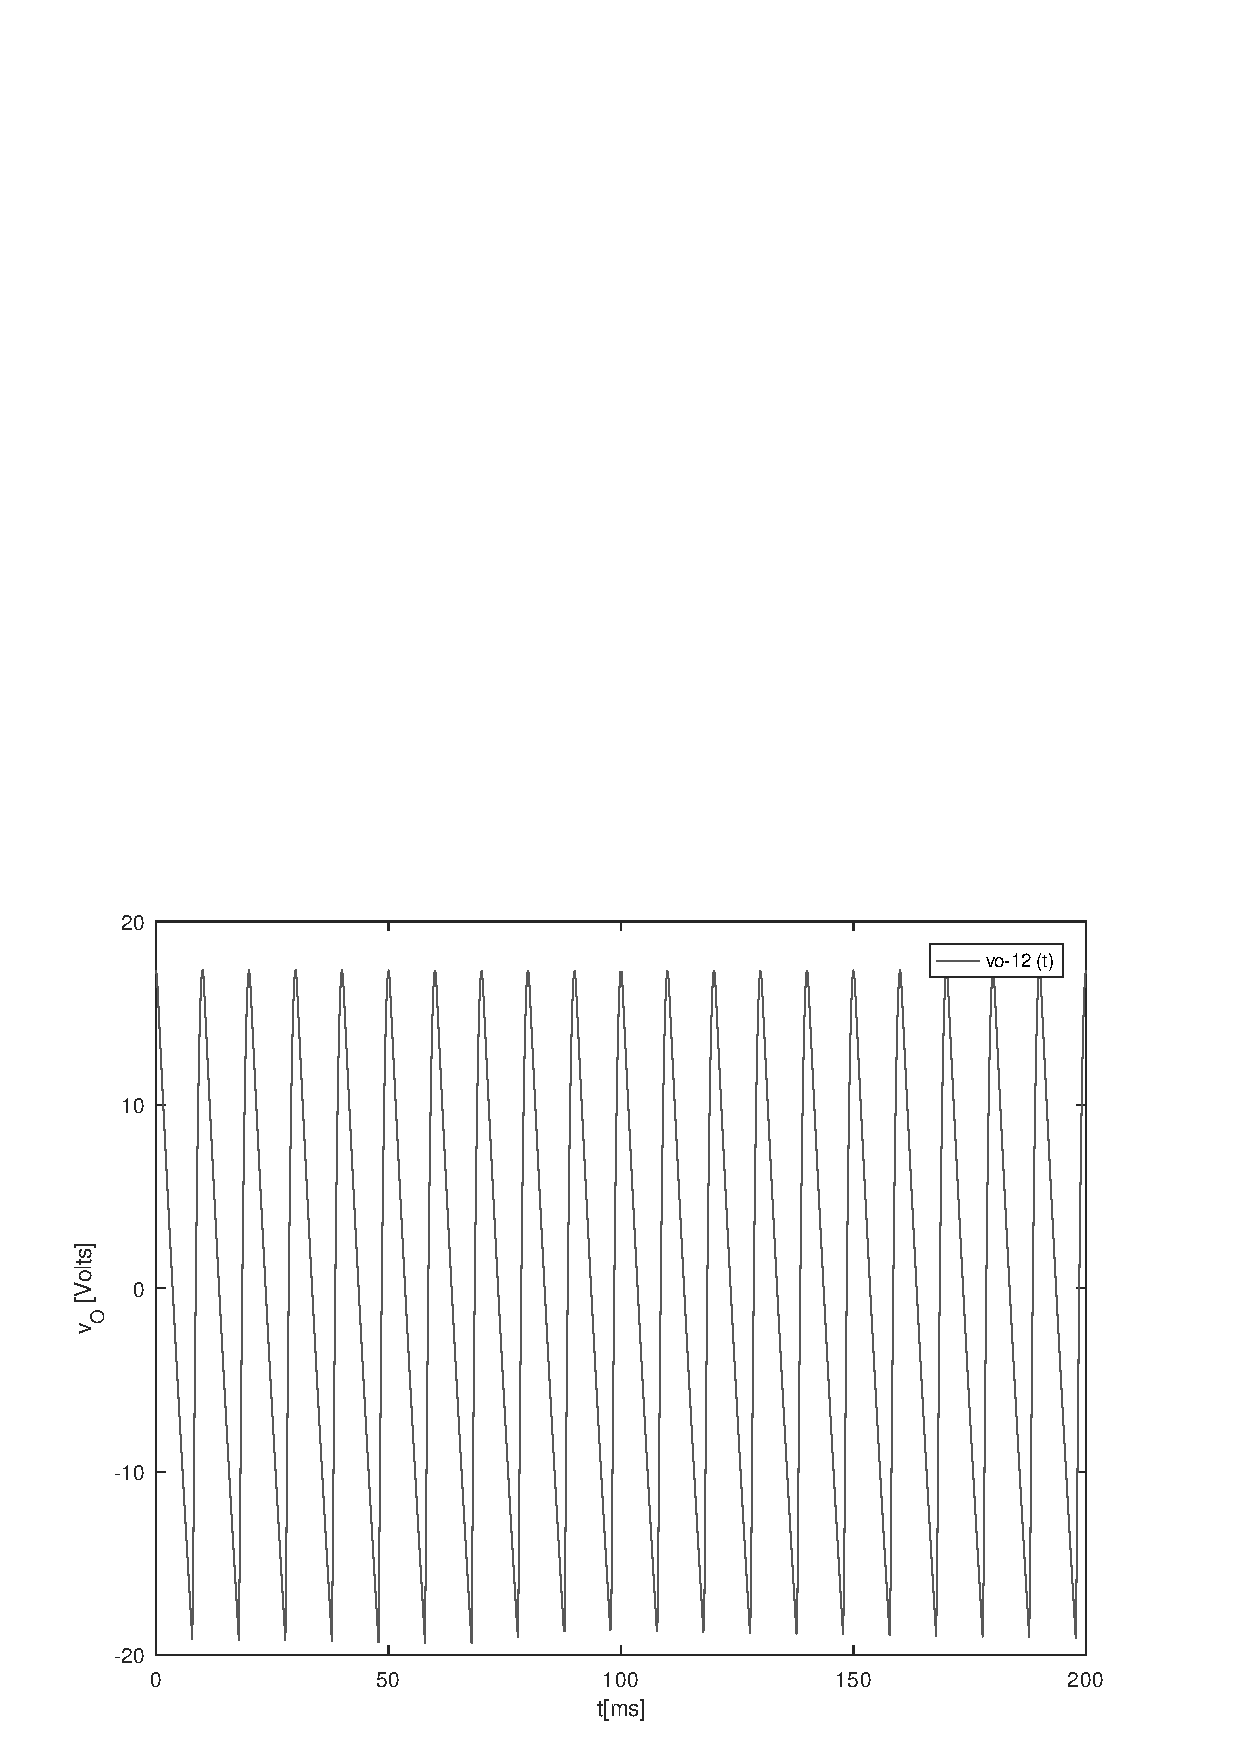
\includegraphics[width=0.8\linewidth]{deviation.pdf}
\label{fig:theo2}
\end{figure}

